\chapter{Results}\label{results}
We evaluate our prototypes using four evaluation criteria: \emph{performance}, \emph{user experience}, \emph{developer experience,} and \emph{security}. Each section in this chapter is dedicated to one criterion.
\section{Performance}\label{results:performance}
We assess the performance of our prototypes for the two test environments, \verb|C++| and \verb|Python|. We first handle the results concerning the implementation details of each prototype. Afterward, we compare them with each other and to the current approach of CodeExpert on the two build cases: first-time and subsequent-time build. We refer in the following to a ``full Nix store'' if we benchmark a subsequent-time build where Nix can use the cached results in the Nix store of the first-time build. An ``empty Nix store'' contains no pre-downloaded binaries of packages.

We made the measurement process of all approaches as comparable as possible by deciding what execution flow resembles the corresponding build case in the best way for each approach. This decision is made separately due to the different implementations and is explained at the beginning of sections \ref{first-time-build} and \ref{subsequent-time-build}. In every benchmark that measures an environment's startup time, the time needed to stop and remove the container is also included in the measured real-time. Therefore the time until the environment is ready to execute the user's code is faster than what was measured.

\subsection{BIAR: approach specific}\label{biar-approach-specific}
For the BIAR approach, we want to determine which strategy (layered or streamed) is better to build images in the builder container and push them to the registry (see \ref{BIAR-components}). We use a registry running inside another container on the same host to simulate the current image registry execution flow of CodeExpert (see \ref{CX-configuration}). We only show the figures of the \verb|Python| environment, as the differences between the strategies are similar for the \verb|C++| environment.

\begin{figure}[h!]
  \centering
  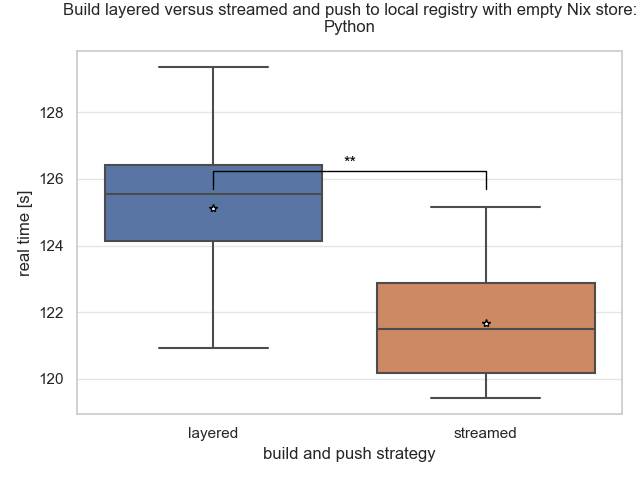
\includegraphics[width=0.71\textwidth]{thesis/graphics/biar-plots/build_layered_versus_streamed_and_push_to_local_registry_with_empty_nix_store:_python.png}
  \caption{Comparing the build and push strategies streamed and layered using an \emph{empty} Nix store. Remarks: * = a higher number of stars(*) indicates a greater statistically significant difference}
  \label{fig:biar-layered-vs-streamed-full-store-python}
\end{figure}

When the Nix store is empty, we observe that streaming is significantly faster for both \verb|Python| and \verb|C++| environments than the layered strategy (see fig. \ref{fig:biar-layered-vs-streamed-empty-store-python}. However, when we used a full cache (Nix store), there was no significant difference between the strategies, as shown in figure \ref{fig:biar-layered-vs-streamed-full-store-python}.

\begin{figure}[h!]
    \centering
  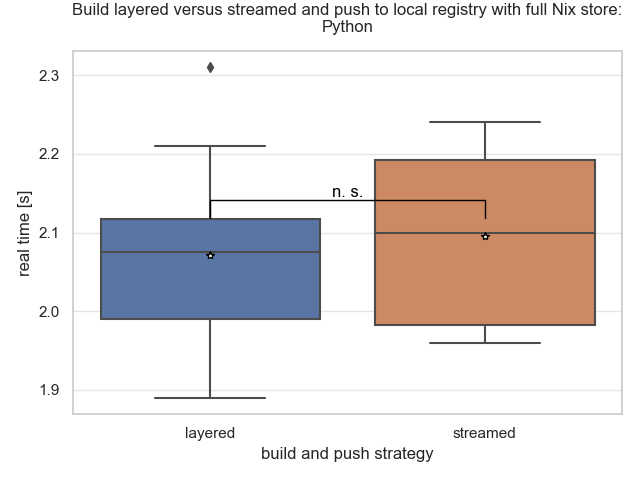
\includegraphics[width=0.71\textwidth]{thesis/graphics/biar-plots/build_layered_versus_streamed_and_push_to_local_registry_with_full_nix_store:_python.png}
  \caption{Comparing the build and push strategies streamed and layered using a \emph{full} Nix store.
  Remarks: n.s. = statistically nonsignificant difference}
  \label{fig:biar-layered-vs-streamed-empty-store-python}
\end{figure}

The measured times are almost identical in the full Nix store case since both strategies use the store as a cache and skip building the image. In this case, the build time is dominated by the time (approx. 2s) it takes to push the layers to the registry. This push time means that even with caching the image built in the builder container, the current prototype's build time is still bounded by the push time. This influenced the prototype's design to skip the push step in \ref{BIAR-execution-flow}. When the cache is empty, the build time is dominated by the building of the image, which takes approx. 120s, and not by the push time, which is only around 2s.

\subsection{NSAR approach specific}
To determine the best internal implementation of the NSAR approach, we show our results of caching the nix-shell and using a seeded Nix store in the following paragraphs.

\paragraph{Caching nix-shell}
We want to test the performance of our idea of caching the nix-shell (see \ref{caching-nix-shell}) with benchmarks. We restrict ourselves to the \verb|C++| environment, as the results are similar to the \verb|Python| environment.

First, we assess the case where the Nix store is full (see fig. \ref{fig:nsar-cached-vs-uncached-full-store-python}), where the environment build-time with the cached nix-shell is almost three times faster than the uncached one. This is because the cached nix-shell can use the cached environment variables and skip the evaluation of the input files. Thus it is faster than the uncached nix-shell. When we assess first-time builds, where the Nix store is initially empty, we observe almost the opposite -- the cached nix-shell is slower than the uncached nix-shell by approx. 20\% (see fig. \ref{fig:nsar-cached-vs-uncached-empty-store-python}). This is because the cache has to be initialized and updated by the cached nix-shell, which incurs some overhead.

\begin{figure}[h!]
    \centering
    \begin{subfigure}{\textwidth}
        \centering
      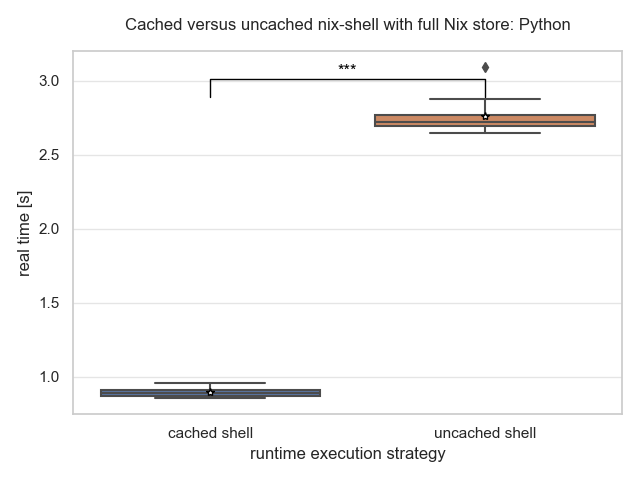
\includegraphics[width=0.75\textwidth]{thesis/graphics/nsar-plots/cached_versus_uncached_nix-shell_with_full_nix_store:_python.png}
      \caption{Comparison using a full Nix store}
      \label{fig:nsar-cached-vs-uncached-full-store-python}
    \end{subfigure}
    \begin{subfigure}{\textwidth}
      \centering
      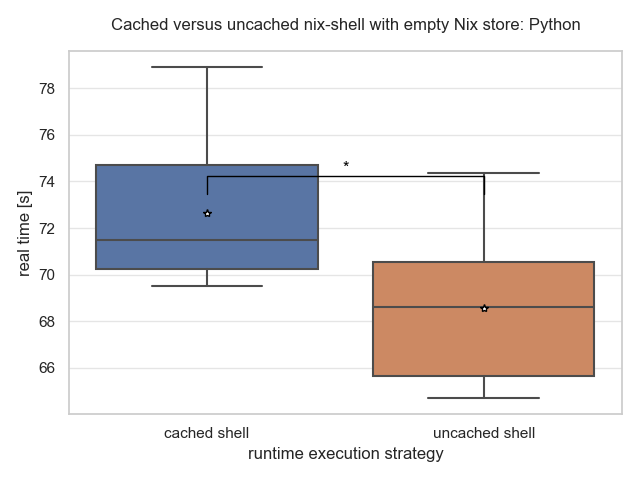
\includegraphics[width=0.75\textwidth]{thesis/graphics/nsar-plots/cached_versus_uncached_nix-shell_with_empty_nix_store:_python.png}
      \caption{Comparison using an empty Nix store}
      \label{fig:nsar-cached-vs-uncached-empty-store-python}
    \end{subfigure} 
    \caption{The ``full store'' is a measurement of a subsequent-time build that uses the cached results of a first-time build with the same configuration. The Nix store is empty for the first-time build. We show the Python environment results. Remarks: cached shell = cached nix-shell (see \ref{caching-nix-shell}), uncached shell = standard nix-shell (see \ref{nix-shell&nix-build}), * = a higher number of stars(*) indicates a greater statistically significant difference.}
    \label{fig:nsar-cached-vs-uncached}
\end{figure}

\paragraph{Seeded store}\label{results-seeded-nix-store}
To determine whether the idea of using a seeded store (see \ref{seeded-nix-store}) improves the performance, we compared it to an empty store and a full store. We prebuild the Nix store with the packages from the $C_{base}$ file as these packages are known at build time and do not depend on the lecturer’s modification. Additionally, we prebuild the Nix store with the packages specified in \ref{appendix:bench-envs-packages} and use a configuration with some additional packages for benchmarking the build time. These additional packages should simulate a configuration modification, where some popular packages are in the seeded store, and the lecturer wants to install some more that are not yet available. We use a cached nix-shell for both comparisons and restrict ourselves to show the \verb|C++| environment here.

\begin{figure}
    \centering
    \begin{subfigure}{\textwidth}
        \centering
      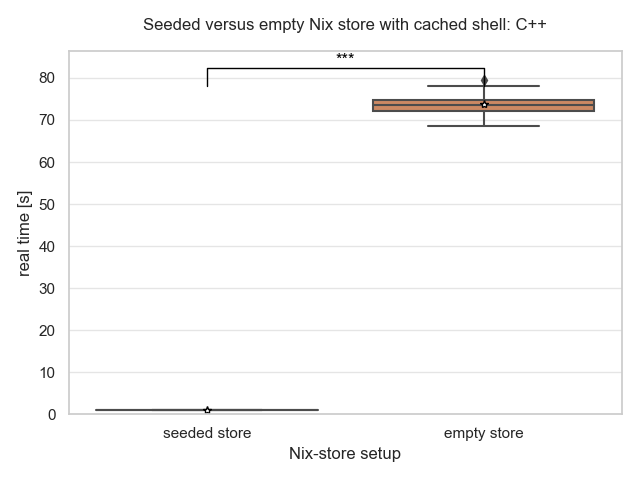
\includegraphics[width=0.75\textwidth]{thesis/graphics/nsar-plots/seeded_versus_empty_nix_store_with_cached_shell:_c++.png}
      \caption{}
      \label{fig:nsar-seeded-vs-empty-store-cpp}
    \end{subfigure}
    \begin{subfigure}{\textwidth}
    \centering
      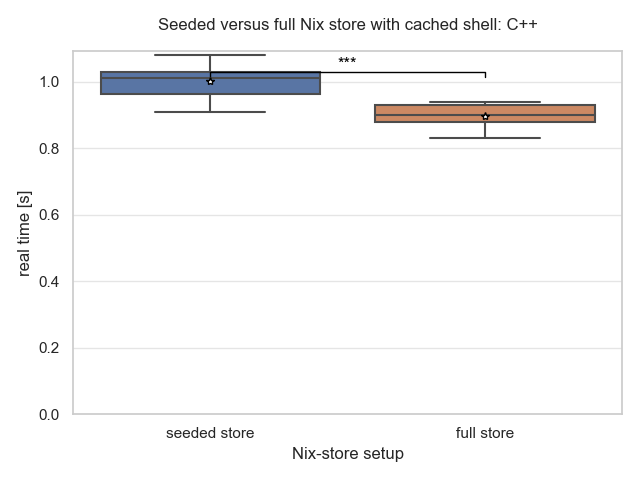
\includegraphics[width=0.75\textwidth]{thesis/graphics/nsar-plots/seeded_versus_full_nix_store_with_cached_shell:_c++.png}
      \caption{}
      \label{fig:nsar-seeded-vs-full-store-cpp}
    \end{subfigure} 
    \caption{The ``seeded store'' has a subset of the packages used to build the measured build time preinstalled. The ``full store'' is a measurement of a subsequent-time build that uses the cached results of a first-time build with the same configuration. We show the \texttt{C++} environment results. Remarks: * = a higher number of stars(*) indicates a greater statistically significant difference.}
    \label{fig:nsar-seeded}
\end{figure}

When comparing the build time of an empty store with that of a seeded store, we can observe that the latter brings an order of magnitude (50x) improvement in performance (see fig. \ref{fig:nsar-seeded-vs-empty-store-cpp}). 

By inspecting figure \ref{fig:nsar-seeded-vs-full-store-cpp}, we note that there is small (approx. 100ms) but signifficant difference when using a seeded store versus a full store. Interestingly when comparing both environments (fig. \ref{fig:nsar-seeded-vs-full-store-cpp} and fig. \ref{appendix:seeded-nix-store-python}) we observe that the \verb|Python| version has a smaller statistical difference (two stars) than the \verb|C++| one (three stars) even though we add 1 \verb|Python| package and 5 OS-packages to the \verb|Python| configuration compared to only 1 additional package in case of the \verb|C++| configuration change (see \ref{appendix:bench-envs-packages}). 


\subsection{First-time build}\label{first-time-build}
The first-time build performance -- starting from the new configuration until the container environment is “ready” -- corresponds to the case where all build-caches are empty. This case happens, for example, when the configuration $C_{result}$ specified by the lecturer is such that no previously cached outputs can be used. We made the measurement process of the approaches as comparable as possible by deciding what execution flow resembles the first-time build in the best way for each approach. This decision is made separately due to the different implementations. We explain how we measured the build time for each approach next.

In the BIAR prototype, we assume that the builder container image is available and the shared Nix store of the builder container is empty. We measure the following steps: start the builder container, then build and push the layered image built from $C_{result}$ as a stream to the registry. Then pull the built image from the registry, and start an environment container from it. 

We measure the build time of the NSAR by assuming that the shared Nix store of the environment container is empty and the minimal base image is cached locally on the container engine host. We measure the following step: start the environment container with the configuration and project files bind-mounted into the container and run the cached nix-shell to build the environment with the packages available. 

In the current CodeExpert approach, the cxEnvrionment image extends the base image \verb|base-rhel8|. We assume this base image is already built, as the lecturer configuration change does not influence it. We measure the following steps: build the cxEnvrionment image, then pull this image from the registry, and start a container from it. We use the \verb|Python-3_8| and \verb|GCC| images and compare them to our \verb|Python| and \verb|C++| environments, respectively. We did not measure the time it takes to push the image to the registry for this approach.

We can start an environment without network access for BIAR and the current approach, unlike the NSAR environments.

\paragraph{Prototypes compared with each other}
Depending on the environment, the NSAR prototype is two to four times faster than the BIAR approach (see figure \ref{fig:nsar-biar-first-time-build-python}). This considerable difference is due to the additional work BIAR does. Both prototypes need to download almost the same packages from the binary cache. However, the BIAR approach must additionally build an image, then push it to and pull it from the registry. Since the significant difference is large for both environments, we only show the \verb|C++| environment’s figure here. 
\begin{figure}
  \centering
  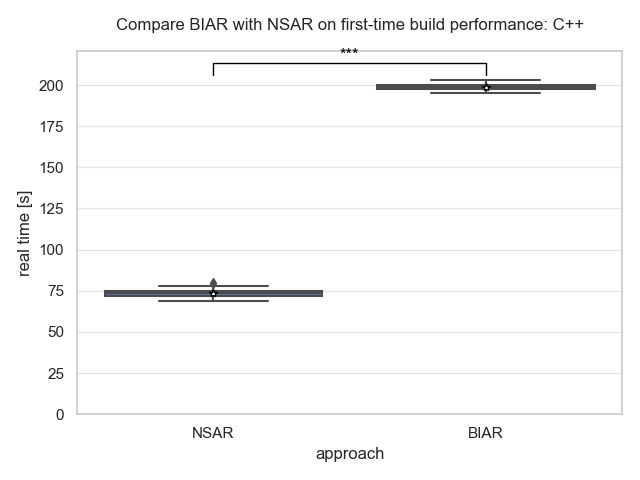
\includegraphics[width=0.75\textwidth]{thesis/graphics/compare-plots/compare_biar_with_nsar_on_first-time_build_performance:_c++.png}
  \caption{Remarks: \texttt{C++} = \texttt{C++} environment, NSAR = nix-shell at runtime, BIAR = build image at runtime, * = a higher number of stars(*) indicates a greater statistically significant difference.}
  \label{fig:nsar-biar-first-time-build-python}
\end{figure}

\paragraph{Prototypes compared to current approach}\label{prototypes-vs-current-first-time-build}
For the \verb|C++| environment, the current approach is slower than NSAR but faster than BIAR (see figure \ref{fig:prototypes-vs-current-first-time-build-cpp}). BIAR and the current approach build the \verb|C++| and GCC image, respectively, using only prebuilt binaries. However, the current approach performs slightly better than BIAR. This difference can have multiple reasons as they most importantly use different image build systems. Additionally, the push time to the registry is missing in the benchmark of the current approach, and the BIAR prototype includes an additional large \verb|C++| package (see \ref{appendix:bench-envs-packages}) in its configuration.

By inspecting figure \ref{fig:prototypes-vs-current-first-time-build-python}, we can note that building the \verb|Python| environment with the current implementation is much slower than both BIAR and NSAR. This is because the current approach builds \verb|Python| from source code, unlike our prototypes that use prebuilt binaries. Therefore we cannot compare the results for this environment.
\begin{figure}
    \centering
    \begin{subfigure}{\textwidth}
        \centering
      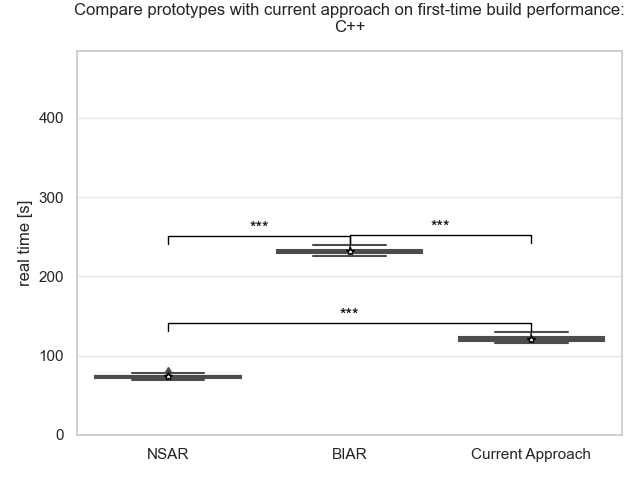
\includegraphics[width=0.87\textwidth]{thesis/graphics/compare-plots/compare_prototypes_with_current_approach_on_first-time_build_performance:_c++.png}
      \caption{\texttt{C++} environment}
      \label{fig:prototypes-vs-current-first-time-build-cpp}
    \end{subfigure}
    
    \vspace{1em}
    \begin{subfigure}{\textwidth}
    \centering
      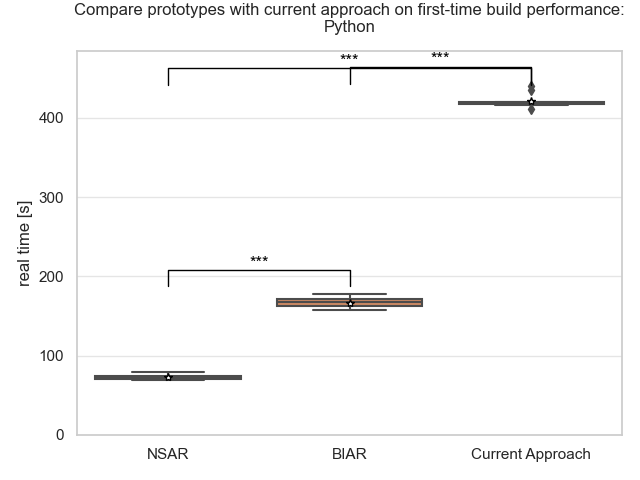
\includegraphics[width=0.87\textwidth]{thesis/graphics/compare-plots/compare_prototypes_with_current_approach_on_first-time_build_performance:_python.png}
      \caption{\texttt{Python} environment}
      \label{fig:prototypes-vs-current-first-time-build-python}
    \end{subfigure}
    \caption{First-time build performance of all approaches compared. Remarks: NSAR = nix-shell at runtime, BIAR = build image at runtime, * = a higher number of stars(*) indicates a greater statistically significant difference.}
    \label{fig:prototypes-vs-current-first-time-build}
\end{figure}

\subsection{Subsequent-time build}\label{subsequent-time-build}
The subsequent-time build (startup) performance -- start an environment container with a previously built configuration $C_{result}$ -- implies that the build-cache is full. The same argumentation for the network access holds as in the first-time build (see \ref{first-time-build}), and we explain how we measured the build time for each approach next.

In the BIAR approach, we assume that the environment image is available on the local container engine host since it has been previously built. The only step we need to do is start the right image inside a container. We find the correct image to start from the given $C_{result}$ by computing the hash over the configuration files before starting the container. 

The NSAR approach assumes that the store of the environment image has all derivations of the configuration installed. The execution flow follows: start a container from the environment image and run the cached nix-shell, which can instantly start the environment shell.

For the current approach, we assume that the environment image is available on the local container engine host. We start the image as a container, and the environment is ready. 
\paragraph{Prototypes compared with each other}
\begin{figure}[h!]
  \centering
  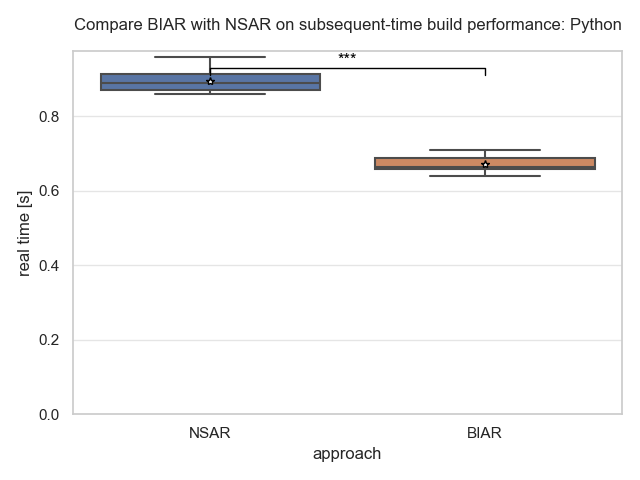
\includegraphics[width=0.74\textwidth]{thesis/graphics/compare-plots/compare_biar_with_nsar_on_subsequent-time_build_performance:_python.png}
  \caption{Comparing the measurements of our prototypes' subsequent-time environment startup performance using the Python environment. Remarks: NSAR = nix-shell at runtime, BIAR = build image at runtime, * = a higher number of stars(*) indicates a greater statistically significant difference.}
  \label{fig:nsar-biar-subsequent-time-build-python}
\end{figure}
We can see in figure \ref{fig:nsar-biar-subsequent-time-build-python} that BIAR is significantly faster than NSAR. BIAR takes between 0.65 and 0.7 seconds, whereas the NSAR startup time lies in the time range of 0.85 to 0.95 seconds. Since both have similar results, we can restrict ourselves to the \verb|Python| environment. This difference is incurred mainly because the NSAR prototype must check if the cache can be reused for the nix-shell execution and bind mounts two additional directories into the container. It also needs network access, which adds overhead as it requires Docker to add network configuration at the environment startup. 

\paragraph{Prototypes compared to current implementation}
The current approach has a startup time of around 0.6 seconds which is significantly faster than both prototypes (around 300ms faster than NSAR and 100ms faster than BIAR). This result can be observed in figure \ref{fig:subsequent-time-build-cpp} and is analogous to the \verb|Python| environment. We already provided some likely causes why NSAR is slower than BIAR. One reason for the difference between BIAR and the current approach might be the former's MD5 hash value computation over the configuration before starting the environment.

\begin{figure}[h!]
  \centering
  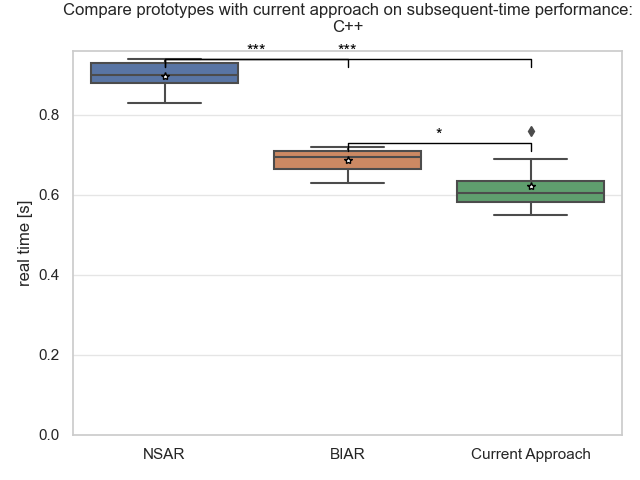
\includegraphics[width=0.8\textwidth]{thesis/graphics/compare-plots/compare_prototypes_with_current_approach_on_subsequent-time_performance:_c++.png}
  \caption{Comparing the measurements of our prototypes' subsequent-time environment startup performance to the current approach using the \texttt{C++} environment. Remarks: NSAR = nix-shell at runtime, BIAR = build image at runtime, * = a higher number of stars(*) indicates a greater statistically significant difference.}
  \label{fig:subsequent-time-build-cpp}
\end{figure}

%\subsection{Scalability}
%We want to benchmark how ``scalable'' an approach is in terms of growing disk space usage as the number of environments users use increases. As each environment in our  

\section{Security}\label{results-security}
The security of an environment is essential as we want to restrict users from breaking out of their isolated container to prevent attacks on the host system or other users' environments. At the same time, we want to provide a controlled and isolated environment to each user for remote code execution because we are in the context of a cloud IDE. 

We assume in this section that beyond the prototype-specific implementation, an environment is implemented such that exploits are made as hard as possible (e.g., remove privileges and access to the kernel). Under this assumption, the current approach is less likely to have security vulnerabilities. 

We discuss the two main attack vectors, the shared cache and network access for both prototypes, and how they could lead to security vulnerabilities. We outline ideas for preventing these vulnerabilities with potential implementations in the further work (see \ref{restrict-network-security} and \ref{improve-shared-cache-security}).

The BIAR prototype is generally vulnerable to attacks from the lecturers as the builder container has both attack vectors. In contrast, the NSAR prototype is vulnerable to attacks from any user since every user interacts with the environments with both attack vectors.

The environments produced by the BIAR prototype have no security vulnerabilities inherent to the implementation. Other vulnerabilities may exist that are not a direct result of our implementation -- for example, insecure packages. We can remove access to the network for each environment, and there is no shared component between containers. 
\subsection{Shared cache attacks}
We divide this section of cross-cache attacks into the two types of shared caches: the Nix store and the nix-shell cache. The latter is only applicable to the NSAR prototype.
\paragraph{Cross-cache attacks on the Nix store}\label{cross-cache-attacks-on-nix-store}
The Nix store cache is vulnerable to denial-of-service (DoS) attacks. For example, a malicious user could fill the cache with garbage derivations until the VM runs out of memory.

In addition, the shared Nix store is possibly vulnerable to cache poisoning. A user can put invalid entries (derivations) into the cache, which another environment container could access and deem valid. For example, a malicious user could construct a derivation that has as directory name the hash of a popular package $p$ and put it inside the store. If a configuration specifies this package $p$ in some following build process, then Nix will use the faulty cached derivation from the shared Nix store.

In our prototypes, the Nix database is also shared. It keeps track of the mapping between dependencies and derivations in the Nix store and can be arbitrarily modified to remap dependencies between derivations. One result is that the database becomes out of sync with the Nix store. Thus the database needs to be rebuilt by Nix if it cannot use the mappings from the database, which degrades performance and could even result in DoS. 

Possibly, the lecturer could introduce unintended security vulnerabilities to an environment, for example, by misconfiguring a package or using a malicious package. It is generally the responsibility of the lecturer to configure an image correctly, but these unintended attack vectors could compromise the Nix store. Nix employs defaults that prevent packages’ installation from the Nixpkgs collection based on the package metadata. Nix will not install a package if its meta value indicates that it is broken, does not run on the given system, or has known security vulnerabilities. 

The multi-user feature (see \ref{Nix-multi-user}) makes some security vulnerabilities harder to exploit (e.g., cache poisoning). This is because the root owns the Nix store and database, and builds are performed by a daemon, preventing arbitrary builds. Thus a user may need root permissions to access and change part of the Nix store and database. However, multi-user mode does not help with other attacks like DoS on the Nix store and does not improve the vulnerable nix-shell cache. The reason for this is that this feature is devised to share the Nix store across multiple user accounts to prevent cross-user attacks, but not share the Nix store across environment containers that all have the same user.
\paragraph{Cross-cache attacks on nix-shell cache}\label{cross-cache-attacks-on-nix-shell-cache}
Environments in the NSAR prototype share two caches, one for the Nix store and the other for the nix-shell. The NSAR approach needs both caches to achieve fast startup times for subsequent environment builds. 

The same security vulnerabilities as for the shared Nix store potentially exist for the nix-shell cache, which currently has no barriers against cross-cache attacks. This is because the files inside the nix-shell cache are writable by the user, unlike the files in the Nix store, which are read-only. Thus a user could quickly delete the cached files, which delays other environments’ startup time, or change the files in arbitrary ways. An example of the latter is changing the symlink of the \verb|nix-shell |’s derivation so that it points to another derivation in the nix store.

\subsection{Network access attacks}\label{security:network-access-attacks}
Each builder container of BIAR or environment of NSAR has access to the public network, mainly to provide the nix-shell access to the binary cache (cache.nixos.org) to download prebuilt packages not already in the Nix store. Another reason to provide network access would be to allow the use of ``fetcher'', which Nix provides to fetch source code from repositories like Github, Gitlab, or PyPI \cite{NixFetchers}. These fetchers are needed if users want to, for example, build specific versions of packages from source code that are not available in the Nixpkgs collection.

Unrestricted network access is problematic as it would allow a user to potentially fetch arbitrary sources such as code repositories or web pages. This broad access would make it significantly easier to execute malicious code remotely to attack the cloud system or, for example, use the computing resources for adverse purposes. Another thing to remark is that in the particular use case of CodeExpert, students are not allowed to access the network, for example, during programming exams. This case is not a security vulnerability per se but a requirement that must be satisfiable for our prototype to be used in this context.

%To summarize this security evaluation, the BIAR prototype has fewer security vulnerabilities than the NSAR one.

\section{User experience}\label{result:UX}
To evaluate if our prototypes boost the flexibility in coding exercises, we evaluate the user experience compared to the current solution. The lecturer must set up the coding environments first such that students can run coding exercises in the environments. Therefore this section covers the process, flexibility, and wait time for setting up a configuration. Additionally, it looks at students' interaction response time for environment startups. %For this section, the user of the BIAR prototype is the lecturer, and the user of the NSAR prototype are all users. 

We define a ``good'' user experience in our context with the following properties that are influenced by the ``user experience'' (UX) concept described in \cite{fagerholm2012}.
\begin{enumerate}
	\item Ease of writing configurations
	\item Flexibility of setting up environments with any language and packages
	\item Efficient change of configurations, which includes the build time of the configuration
	\item Quick environment startup times for subsequent environment startups
\end{enumerate}

\subsection{Configuration}\label{user-experience-config}
We first cover the identical arguments for our prototypes because both use Nix as a build system. With the BIAR and NSAR prototypes, the lecturers can directly specify all environment packages themselves (without interacting with the developer) by changing one of the configurations of $C_{preset}$. Such a configuration has a fixed interface (see \ref{prototype-configuration}) for increasing the ease of use when writing configurations. Changing the configuration for lecturers that only specify packages from the Nixpkgs collection is trivial, as the lecturers do not need to learn the Nix language. To showcase the ease of specifying and changing the configuration, one can look at the \nameref{preset-python.nix} configuration and compare it to the \nameref{changed-python.nix} configuration. The \nameref{preset-python.nix} is a reduced example from $C_{preset}$. One Python package and two other packages have been added as highlighted in \nameref{changed-python.nix}.
\definecolor{light-gray}{gray}{0.75}
\begin{lstlisting}[caption={preset-python.nix}, title={preset-python.nix}, label={preset-python.nix}]
{ pkgs }: with pkgs;
let
  pythonEnv = python39.withPackages (p: with p; [
    numpy
  ]);
in
{ inputs = [ pythonEnv ]; }
\end{lstlisting}
\begin{lstlisting}[caption={changed-python.nix}, title={changed-python.nix}, label={changed-python.nix}, escapechar=!]
{ pkgs }: with pkgs;
let
  pythonEnv = python39.withPackages (p: with p; [
    numpy
    !\colorbox{light-gray}{networkx}!
  ]);
in
{ inputs = [ pythonEnv !\colorbox{light-gray}{openssl}! !\colorbox{light-gray}{sqlite}! ]; }
\end{lstlisting}
If the lecturer wants to specify a custom package or package version, then he needs to learn some details of the Nix language for declaring the package as a derivation. Specifying a custom derivation can be challenging, but there are many examples in the Nix documentation (e.g., \cite{NixPythonGuide}) which should provide ample resources for this task. With some packages and languages, the lecturer may need to figure out which environment variables need to be set at runtime, e.g., such that the compiler finds the shared libraries for linking. This can be challenging, but there are many examples of typical use cases in the Nix documentation, e.g., in \cite{NixPythonGuide}. The NSAR prototype makes the specification and restriction of global environment variables inside the shell easy and has a \verb|shellHook| attribute in the configuration interface for this purpose. This specification and restriction of environment variables may be more challenging with the BIAR prototype as environments do not have the \verb|nix-shell| functionality. Special attention is needed when configuring interpreted language using our prototypes. Nix wraps one interpreter and other executables together such that they can find each other and all of the modules. Thus Nix only allows one of these wrapped environments to be installed globally since they otherwise conflict with the interpreter to load out of the PATH environment variable \cite{NixPythonGuide}.

In the current solution, the lecturer cannot deploy the configuration changes directly and must contact the developer to deploy every (minor) change in the configuration. This process can sometimes be advantageous for the lecturer since the developer is responsible for making the images run correctly in production. On the flip side, it may also happen that the developer cannot make a (small) configuration change requested by the lecturer as it may be, e.g., too tricky. If the lecturer does not want to use a predefined configuration, he can write his custom configuration or extend a predefined configuration. This requires knowledge of writing a \verb|Dockerfile| \cite{CXDocs}. Unlike our prototypes which allow the composition of configurations, in most cases, the lecturer cannot easily compose two different configurations written as \verb|Dockerfile|'s into one image in the current solution as argued in \ref{reproducibility-docker-build}.

\subsection{Flexibility}
The current solution restricts the lecturers to packages and specific versions that are available in the used Linux distribution, such that it may happen that a package requested by the lecturer is not available for installation. With our prototypes, lecturers can choose from over 60'000 predefined packages from the Nixpkgs collection or declare any custom package or version they need. This is because Nix can build a package from source code by fetching this code from remote code repositories. The result is almost unlimited flexibility for configuring the environment. 

\subsection{Wait time for user interactions}
This section discusses the time the user must wait until different interactions (e.g., changing the configuration) are complete with our environments. 

The faster the build time, the quicker the lecturer can iterate over configurations during development and when changing the configuration, which improves the UX. Therefore we use the results from \ref{prototypes-vs-current-first-time-build} to evaluate the efficiency of configuration changes. The build time for BIAR is approx. between 2 and 4 min, which is slower than NSAR, which takes around 1min for a complete build with empty caches. Note that after some packages have been built, the build caches are unlikely to be empty, and the build times tend to be faster. Furthermore, both of our approaches allow us to significantly optimize the first-time build performance with a seeded store in the case of NSAR (see \ref{results-seeded-nix-store}) and in the case of BIAR see \ref{optimize-build-and-push-BIAR}.

The current solution has a bit faster build time than BIAR but is slower than NSAR. However, with the current solution, the lecturer only reaches these build times when testing the environment on a local machine. In contrast, our approaches allow direct testing on production systems after the above build time. To test a configuration change with the current approach in the cloud system, the lecturers must contact the developer. Then he must wait potentially many days until the developer has deployed the corresponding image to use it.

The other primary user interaction with our environment that incurs wait time is when a student wants to run coding exercises. In this case, the first student who starts an environment from a new configuration must wait longer, whereas all following students experience the subsequent startup time. Since students invoke an environment startup many times for each job execution, the faster the subsequent startup time, the better the UX. Note that the current solution is faster than BIAR, which is faster than NSAR (see \ref{subsequent-time-build}). 

%TODO: maybe include this in the discussion?
%\subsection{Security of builds and environments}
%Students who run code inside environments and lecturers who configure coding exercises are interested in secure environments and isolated builds from other users, respectively, for a good UX. As argued in section (\ref{results-security} this property is not satisfied for any user in the NSAR prototype nor for the students in the BIAR prototype.

To summarize the UX of the lecturer, our approaches have advantages in configuration, flexibility, and build time over the current solution. On the other hand, the current solution has the edge in the subsequent startup performance for students. 

\section{Developer experience}\label{result:DevX}
In this section, we evaluate the developer's experience in maintaining and developing the implementation of our prototypes compared to the current approach.

We define a ``good'' developer experience for our problem with the following properties influenced by CodeExpert developer's feedback and the developer experience defined in \cite{fagerholm2012}.
\begin{enumerate}
	\item Minimal workload from configuration changes by the lecturer
	\item Less responsibility for usage defects
	\item Ease of development and testing 
	\item Minimal maintenance of implementation (e.g., images and dependencies)
	\item Increase robustness of the cloud-based system.
\end{enumerate}

\subsection{Developer involvement with configuration changes}
Ideally, the developer does not need to be involved whenever a lecturer submits a new or changed configuration for deployment on the production systems. This goal minimizes the developer's workload and is fulfilled with our prototypes. This stands in contrast to the current approach, where the developer needs to be in direct contact with the lecturer and perform the following manual steps
\begin{itemize}
	\item check if the requested packages are available for installation,
	\item figure out how these packages need to be installed,
	\item if they can be installed without much difficulty, then build and then test the image,
	\item and if all the above steps are successful, deploy it to the image registry.
\end{itemize}

Another critical point is that our approaches shift the responsibility for setting up a correct and secure image (e.g., not using broken or vulnerable packages) from the developer to the lecturer. This argument follows from the above argumentation, where we outline the impact of a configuration change on a developer. 

\subsection{Development and testing}
With our prototypes, a developer can easily add, e.g., a new language as a configuration to the $C_{preset}$ group by writing a new template as a Nix expression. This template can then be used or customized by a lecturer. At the moment, adding a new predefined configuration means writing a custom \verb|Dockerfile| and then manually building it and deploying it to the production system, which can be cumbersome.

The developer needs to learn how Nix works and its domain-specific programming language to implement our prototypes, develop them further and test them. Learning Nix can be challenging since it is a purely functional programming language with limited documentation and usage examples. Nix also differs from other functional programming languages such as Haskell. It is often unclear what the ``standard'' Nix approach for a common problem is. However, it is generally advisable to use and compose the many predefined helper functions from the standard library. To aid with development, Nix provides a repl tool that is useful for trying out small Nix code examples and the nix-shell that allows for incremental builds and debugging inside the build-environment (see \ref{nix-shell&nix-build}). 

Nix provides tools that make debugging more manageable: the nix-shell sets up the build environment that can be debugged and inspected and from which the developer can build the package or image manually. Testing container images is best done in a continuous integration (CI) pipeline by, for example, building the reproducible images and then running tests specified, e.g., with a bash script. The primary tool to aid with CI and testing in the Nix ecosystem is Hydra (see \cite{Hydra}), which can cache CI builds and make subsequent pipeline runs faster. Furthermore, testing one or two base images of our approaches that rarely change is likely less of a burden to the developer than testing more than a dozen, each with different languages, in the current approach. 

\subsection{Maintenance}
For the NSAR prototype, the developer only needs to maintain a single image, i.e., built with Nix. However, the Nix store needs maintenance as the developer needs to run the garbage collection or store path optimization regularly to avoid running out of disk space. When the developer runs the garbage collection tool of the Nix store, it is essential not to remove potential configuration files (e.g., shell scripts) stored in the Nix store. These files are needed for the container at runtime. Additionally, the nix-shell cache could need maintenance for the NSAR prototype. 

The NSAR prototype has the \verb|cached-nix-shell| package as a dependency, a Nix package developed by the community that needs to be updated by the developer and might break after an update. Adding features to this package or making changes might make maintaining this dependency a burden. However, our prototypes have much fewer dependencies to maintain than the current approach, which has many packages in multiple image configurations with different package managers such as pip and DNF. The fewer dependencies our prototypes have on external packages, the better the developer experience.

The BIAR prototype has two images that the developer needs to maintain and a shared Nix store, where the same arguments apply as described for the NSAR prototype. Because the BIAR prototype builds an image for every unique configuration, the image registry likely becomes overloaded with many images. Therefore it is necessary to remove images from the registry regularly. It would be best to remove the least used images to prevent unnecessary rebuilds, but this would require collecting image usage statistics.

Our prototypes use a specific version of Nixpkgs and Nix, which needs to be updated in the future and would require a rebuild of the images. For the current prototypes, updating the Nix version would imply updating the Nix base image from Docker Hub. Updating the Nixpkgs version is handled using the Nix package \verb|niv|.

It is crucial for an approach's development and robustness that the same build inputs lead to the same output in future builds. The builds of both prototypes produce the same output because they are reproducible, except if the developer changes the configuration or script files that are copied into the image or bind-mounted into the environment. On the other hand, the current approach is not reproducible since the image builds can fail (see \ref{reproducibility-docker-build}). %Furthermore, the current approach has many images which need to be maintained and updated, resulting in a worse developer experience. 

%The developer is interested in the secure implementation of an approach to prevent attacks on the host system. This property is currently not fully satisfied by both of our prototypes, but the BIAR prototype has the advantage over the NSAR prototype. 
